
\subsection{Tucker Decomposition}
The Tucker decomposition \cite{tucker1966some} factorizes a $N$-th order tensor
into smaller tensor and factor matrices. In this decomposition, the smaller
tensor is called the \emph{core tensor}. The Tucker
decomposition consists of $N$ mode-$n$ products (see, e.g., Section~\ref{sec:product})
between the core tensor and the factor matrices.

Let $\Tt \in \RR^{d_1 \times \dots \times d_N}$. A Tucker decomposition of $\Tt$
is given by
\[
    \Tt
    = \Gt \times_1 \Ub_1 \times_2 \Ub_2\times_3 \dots \times_N \Ub_N,
\]
where $\Gt \in \RR^{R_1 \times \dots \times R_N}$ is the core tensor and
$\Ub_i \in \RR^{d_i \times R_i}$ for $i \in [N]$ are the factor matrices.
The $N$-tuple $(R_1,\dots,R_N)$ is called the \emph{rank} of Tucker
decomposition.

The Tucker decomposition of a fourth-order tensor $\Tt\in\RR^{d_1\times\cdots \times d_4}$ can be illustrated using tensor networks notation as follows.
$$
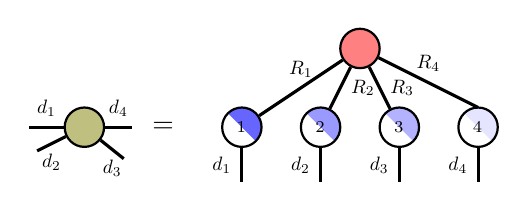
\begin{tikzpicture}[baseline=-0.5ex]
    \tikzset{tensor/.style = {minimum size = 0.5cm,shape = circle,thick,draw=black,inner sep = 0pt}, edge/.style = {thick,line width=.4mm},every loop/.style={}}
    \def\x{6}
    \def\y{0}   \node[tensor,fill=green!50!red!50!white] (T) at (\x+1,\y) {$\Tt$};
    \draw[edge] (T) -- (\x+0.3,0) node [midway,above] {\scalebox{0.7}{\dimcolor{$d_1$}}};
    \draw[edge] (T) -- (\x+1.6,0) node [midway,above] {\scalebox{0.7}{\dimcolor{$d_4$}}};;
    \draw[edge] (T) -- (\x+0.4,-0.3) node [midway, below] {\scalebox{0.7}{\dimcolor{$d_2$}}};
    \draw[edge] (T) -- (\x+1.5,-0.4)node [midway, below] {\scalebox{0.7}{\dimcolor{$d_3$}}};
    \node[draw = none] at (\x+2,0){$=$};
\node[tensor,fill=red!50!white] (G) at (\x+4.5,\y+1) {$\Gt$};
    \node[tensor, path picture={
    \fill[fill=blue!60!white](path picture bounding box.south east)
    -- 
    (path picture bounding box.north west) --
    (path picture bounding box.north east) -- cycle;
    }, shift={(\x+3,\y)}] (U_1) {\scalebox{0.85}{$\Ub_1$}};
    \node[tensor, path picture={
    \fill[fill=blue!40!white](path picture bounding box.south east)
    -- 
    (path picture bounding box.north west) --
    (path picture bounding box.north east) -- cycle;
    }, shift={(\x+4,\y)}] (U_2) {\scalebox{0.85}{$\Ub_2$}};
    \node[tensor, path picture={
    \fill[fill=blue!30!white](path picture bounding box.south east)
    -- 
    (path picture bounding box.north west) --
    (path picture bounding box.north east) -- cycle;
    }, shift={(\x+5,\y)}] (U_3) {\scalebox{0.85}{$\Ub_3$}};
    \node[tensor, path picture={
    \fill[fill=blue!10!white](path picture bounding box.south east)
    -- 
    (path picture bounding box.north west) --
    (path picture bounding box.north east) -- cycle;
    }, shift={(\x+6,\y)}] (U_4) {\scalebox{0.85}{$\Ub_4$}};
    \draw[edge] (G) -- (U_1) node [midway, above] {\scalebox{0.7}{\dimcolor{$R_1$}}};
    \draw[edge] (G) -- (U_2) node [midway, right] {\scalebox{0.7}{\dimcolor{$R_2$}}};
    \draw[edge] (G) -- (U_3) node [midway, right] {\scalebox{0.7}{\dimcolor{$R_3$}}};
    \draw[edge] (G) -- (\x+6,\y+0.25) node [midway, above] {\scalebox{0.7}{\dimcolor{$R_4$}}};
    \draw[edge] (U_1) -- (\x+3,\y-0.7) node [midway, left] {\scalebox{0.7}{\dimcolor{$d_1$}}};
    \draw[edge] (U_2) -- (\x+4,\y-0.7) node [midway, left] {\scalebox{0.7}{\dimcolor{$d_2$}}};
    \draw[edge] (U_3) -- (\x+5,\y-0.7) node [midway, left] {\scalebox{0.7}{\dimcolor{$d_3$}}};
    \draw[edge] (U_4) -- (\x+6,\y-0.7) node [midway, left] {\scalebox{0.7}{\dimcolor{$d_4$}}};
\end{tikzpicture}.
$$


It is not difficult to show that the factor matrices
$\Ub_i \in \RR^{d_i \times R_i}$ can always be chosen to be unitary (see
item~\ref{item:Tucker_orth} in Remark~\ref{rem:tuckers} below).


\paragraph{Multi-linear rank} The \emph{multi-linear (or Tucker) rank}\footnote{Note the distinction between the rank $(R_1,\dots,R_n)$ of a Tucker \emph{decomposition},
given by the size of the core tensor $\Gt$ appearing in
$\Tt = \Gt \times_1 \Ub_1 \times_2 \dots \times_N \Ub_N$, and the
(Tucker) multi-linear rank of a tensor $\Tt$, which is defined as the
minimal such tuple.} of a tensor $\Tt$ is the smallest tuple $(R_1,\dots,R_N)$
for which there exists a rank-$(R_1,\dots,R_N)$ decomposition of $\Tt$. Since there is only 
a partial order on tuples of integers, one may ask whether this notion of rank is well defined. 
The following proposition shows that it is. 

\begin{proposition}
Let $\Tt = \Gt \times_1 \Ub_1 \times_2 \Ub_2\times_3\dots \times_N \Ub_N$ and 
$\Tt = \tilde\Gt \times_1 \tilde\Ub_1 \times_2 \tilde\Ub_2\times_3 \dots \times_N \tilde\Ub_N$ be two 
Tucker decompositions of the same tensor $\Tt$ of rank-$(R_1,R_2,\dots, R_n)$ and 
$(\tilde R_1,\tilde R_2,\dots,\tilde R_n)$, respectively. Then $\Tt$ admits a Tucker decomposition of rank-$(\min(R_1,\tilde R_1), \min(R_2,\tilde R_2), \dots, \min(R_N,\tilde R_N))$. 
\end{proposition}
\begin{proof}
Suppose $N=3$. Applying the mode-$1$ unfolding and Theorem~\ref{thm: matricization-rank} to each of the two Tucker decompositions of $\Tt$ we obtain the following:
\begin{align*}
    \rank\left(\begin{tikzpicture}[baseline=\baseline]
    \tikzset{tensor/.style = {minimum size = 0.5cm,shape = circle,thick,draw=black,inner sep = 0pt}, edge/.style  = {thick,line width=.4mm},every loop/.style={}}
    \def\y{0}
    \def\x{0}
    \node[tensor,fill=green!50!red!50!white] (Tt) at (\x,\y){\scalebox{0.85}{$\Tt$}};
    \draw[edge] (\x+0.25,\y) -- (\x+0.6,\y)  node [midway,above] {\scalebox{0.7}{\dimcolor{$d_2$}}};
    \draw[edge] (\x-0.25,\y) -- (\x-0.6,\y)  node [midway,above] {\scalebox{0.7}{\dimcolor{$d_1$}}};
    \draw[edge] (\x,\y-0.25) -- (\x,\y-0.7)  node [midway,left] {\scalebox{0.7}{\dimcolor{$d_3$}}};
    \end{tikzpicture}\right)_{(1)}
=
\rank(\begin{tikzpicture}[baseline=\baseline]
    \tikzset{tensor/.style = {minimum size = 0.5cm,shape = circle,thick,draw=black,inner sep = 0pt}, edge/.style  = {thick,line width=.4mm},every loop/.style={}}
    \def\y{0}
    \def\x{0}
    \node[tensor,fill=green!50!red!50!white] (Tt) at (\x,\y){\scalebox{0.85}{$\Tt$}};
    \draw[edge] (Tt) -- (\x-0.6,\y)  node [midway,above] {\scalebox{0.7}{\dimcolor{$d_1$}}};
    \draw[edge] (Tt) -- (\x+0.6,\y)  node [midway,above] {\scalebox{0.7}{\dimcolor{$d_2$}}};    \draw[edge] (Tt) -- (\x+0.6,\y)  node [midway,above] {\scalebox{0.7}{\dimcolor{$d_2$}}};
    \draw[edge] (\x+0.25,\y-0.1) -- (\x+0.6,\y-0.1)  node [midway,below] {\scalebox{0.7}{\dimcolor{$d_3$}}};
\end{tikzpicture})
=
\rank\left(\begin{tikzpicture}[baseline=\baseline]
    \tikzset{tensor/.style = {minimum size = 0.5cm,shape = circle,thick,draw=black,inner sep = 0pt}, edge/.style   = {thick,line width=.4mm},every loop/.style={}}
    \def\y{0}
    \def\x{0}
    \node[tensor,fill=blue!60!white] (U_1) at (\x,\y){\scalebox{0.85}{$\Ub_1$}};
    \node[tensor,fill=blue!30!white] (U_2) at (\x+2.7,\y+0.7){$\Ub_2$};
    \node[tensor,fill=blue!10!white] (U_3) at (\x+2.7,\y-0.7){$\Ub_3$};
    \node[tensor,fill=red!60!white] (m) at (\x+1,\y) {$\Gt$}; 
     \draw[edge] (\x+1.2,\y+0.15) -- (\x+1.5,\y+0.15)-- (\x+1.5,\y+0.05) -- (\x+2,\y+0.05) node [midway,above]
    {\scalebox{0.7}{\dimcolor{$R_2$}}};
    \draw[edge] (\x+1.2,\y-0.15) -- (\x+1.5,\y-0.15)-- (\x+1.5,\y-0.05)-- (\x+2,\y-0.05) node [midway,below]
    {\scalebox{0.7}{\dimcolor{$R_3$}}};
    \draw[edge] (U_1) -- (m) node [midway,above] {\scalebox{0.7}{\dimcolor{$R_1$}}};
    \draw[edge] (U_1) -- (\x-0.7,\y) node [midway,above] {\scalebox{0.7}{\dimcolor{$d_1$}}};
    \draw[edge](\x+2,\y-0.05) -- (\x+2,\y-0.7) -- (U_3);
    \draw[edge](\x+2,\y+0.05) -- (\x+2,\y+0.7) -- (U_2);
    \draw[edge] (U_2) -- (\x+3.5,\y+0.7) -- (\x+3.5,\y+0.05)-- (\x+4,\y+0.05) node [midway,above]
    {\scalebox{0.7}{\dimcolor{$d_2$}}};
    \draw[edge] (U_3) -- (\x+3.5,\y-0.7) -- (\x+3.5,\y-0.05) -- (\x+4,\y-0.05) node [midway,below]
    {\scalebox{0.7}{\dimcolor{$d_3$}}};
    \draw[dotted] (\x+0.45,\y+1) -- (\x+0.45,\y-1);
    \end{tikzpicture}\right)\leq R_1,
\end{align*}
and at the same time
\begin{align*}
    \rank\left(\begin{tikzpicture}[baseline=\baseline]
    \tikzset{tensor/.style = {minimum size = 0.5cm,shape = circle,thick,draw=black,inner sep = 0pt}, edge/.style  = {thick,line width=.4mm},every loop/.style={}}
    \def\y{0}
    \def\x{0}
    \node[tensor,fill=green!50!red!50!white] (Tt) at (\x,\y){\scalebox{0.85}{$\Tt$}};
    \draw[edge] (\x+0.25,\y) -- (\x+0.6,\y)  node [midway,above] {\scalebox{0.7}{\dimcolor{$d_2$}}};
    \draw[edge] (\x-0.25,\y) -- (\x-0.6,\y)  node [midway,above] {\scalebox{0.7}{\dimcolor{$d_1$}}};
    \draw[edge] (\x,\y-0.25) -- (\x,\y-0.7)  node [midway,left] {\scalebox{0.7}{\dimcolor{$d_3$}}};
    \end{tikzpicture}\right)_{(1)}
=
\rank(\begin{tikzpicture}[baseline=\baseline]
    \tikzset{tensor/.style = {minimum size = 0.5cm,shape = circle,thick,draw=black,inner sep = 0pt}, edge/.style  = {thick,line width=.4mm},every loop/.style={}}
    \def\y{0}
    \def\x{0}
    \node[tensor,fill=green!50!red!50!white] (Tt) at (\x,\y){\scalebox{0.85}{$\Tt$}};
    \draw[edge] (Tt) -- (\x-0.6,\y)  node [midway,above] {\scalebox{0.7}{\dimcolor{$d_1$}}};
    \draw[edge] (Tt) -- (\x+0.6,\y)  node [midway,above] {\scalebox{0.7}{\dimcolor{$d_2$}}};    \draw[edge] (Tt) -- (\x+0.6,\y)  node [midway,above] {\scalebox{0.7}{\dimcolor{$d_2$}}};
    \draw[edge] (\x+0.25,\y-0.1) -- (\x+0.6,\y-0.1)  node [midway,below] {\scalebox{0.7}{\dimcolor{$d_3$}}};
\end{tikzpicture})
=
\rank\left(\begin{tikzpicture}[baseline=\baseline]
    \tikzset{tensor/.style = {minimum size = 0.5cm,shape = circle,thick,draw=black,inner sep = 0pt}, edge/.style   = {thick,line width=.4mm},every loop/.style={}}
    \def\y{0}
    \def\x{0}
    \node[tensor,fill=red!60!blue!20!white] (U_1) at (\x,\y){\scalebox{0.85}{$\tilde{\Ub}_1$}};
    \node[tensor,fill=red!30!blue!50!white] (U_2) at (\x+2.7,\y+0.7){$\tilde{\Ub}_2$};
    \node[tensor,fill=red!20!blue!40!white] (U_3) at (\x+2.7,\y-0.7){$\tilde{\Ub}_3$};
    \node[tensor,fill=red!40!white] (m) at (\x+1,\y) {$\tilde{\Gt}$}; 
     \draw[edge] (\x+1.2,\y+0.15) -- (\x+1.5,\y+0.15)-- (\x+1.5,\y+0.05) -- (\x+2,\y+0.05) node [midway,above]
    {\scalebox{0.7}{\dimcolor{$\tilde{R}_2$}}};
    \draw[edge] (\x+1.2,\y-0.15) -- (\x+1.5,\y-0.15)-- (\x+1.5,\y-0.05)-- (\x+2,\y-0.05) node [midway,below]
    {\scalebox{0.7}{\dimcolor{$\tilde{R}_3$}}};
    \draw[edge] (U_1) -- (m) node [midway,above] {\scalebox{0.7}{\dimcolor{$\tilde{R_1}$}}};
    \draw[edge] (U_1) -- (\x-0.7,\y) node [midway,above] {\scalebox{0.7}{\dimcolor{$d_1$}}};
    \draw[edge](\x+2,\y-0.05) -- (\x+2,\y-0.7) -- (U_3);
    \draw[edge](\x+2,\y+0.05) -- (\x+2,\y+0.7) -- (U_2);
    \draw[edge] (U_2) -- (\x+3.5,\y+0.7) -- (\x+3.5,\y+0.05)-- (\x+4,\y+0.05) node [midway,above]
    {\scalebox{0.7}{\dimcolor{$d_2$}}};
    \draw[edge] (U_3) -- (\x+3.5,\y-0.7) -- (\x+3.5,\y-0.05) -- (\x+4,\y-0.05) node [midway,below]
    {\scalebox{0.7}{\dimcolor{$d_3$}}};
    \draw[dotted] (\x+0.45,\y+1) -- (\x+0.45,\y-1);
    \end{tikzpicture}\right)\leq \tilde{R}_1,
\end{align*}
Therefore, $\rank\left(\begin{tikzpicture}[baseline=\baseline]
    \tikzset{tensor/.style = {minimum size = 0.5cm,shape = circle,thick,draw=black,inner sep = 0pt}, edge/.style  = {thick,line width=.4mm},every loop/.style={}}
    \def\y{0}
    \def\x{0}
    \node[tensor,fill=green!50!red!50!white] (Tt) at (\x,\y){\scalebox{0.85}{$\Tt$}};
    \draw[edge] (\x+0.25,\y) -- (\x+0.6,\y)  node [midway,above] {\scalebox{0.7}{\dimcolor{$d_2$}}};
    \draw[edge] (\x-0.25,\y) -- (\x-0.6,\y)  node [midway,above] {\scalebox{0.7}{\dimcolor{$d_1$}}};
    \draw[edge] (\x,\y-0.25) -- (\x,\y-0.7)  node [midway,left] {\scalebox{0.7}{\dimcolor{$d_3$}}};
\end{tikzpicture}\right)_{(1)}\leq\min(R_1,\tilde{R}_1)$. 
Applying the same reasoning for $n=2,3$ we conclude that $\Tt$ admits a Tucker decomposition of rank-$(\min(R_1,\tilde{R}_1),\min(R_2,\tilde{R}_2),\min(R_3,\tilde{R}_3))$.
\end{proof}

